\documentclass[11pt]{article}

    \usepackage[breakable]{tcolorbox}
    \usepackage{parskip} % Stop auto-indenting (to mimic markdown behaviour)
    
    \usepackage{iftex}
    \ifPDFTeX
    	\usepackage[T1]{fontenc}
    	\usepackage{mathpazo}
    \else
    	\usepackage{fontspec}
    \fi

    % Basic figure setup, for now with no caption control since it's done
    % automatically by Pandoc (which extracts ![](path) syntax from Markdown).
    \usepackage{graphicx}
    % Maintain compatibility with old templates. Remove in nbconvert 6.0
    \let\Oldincludegraphics\includegraphics
    % Ensure that by default, figures have no caption (until we provide a
    % proper Figure object with a Caption API and a way to capture that
    % in the conversion process - todo).
    \usepackage{caption}
    \DeclareCaptionFormat{nocaption}{}
    \captionsetup{format=nocaption,aboveskip=0pt,belowskip=0pt}

    \usepackage[Export]{adjustbox} % Used to constrain images to a maximum size
    \adjustboxset{max size={0.9\linewidth}{0.9\paperheight}}
    \usepackage{float}
    \floatplacement{figure}{H} % forces figures to be placed at the correct location
    \usepackage{xcolor} % Allow colors to be defined
    \usepackage{enumerate} % Needed for markdown enumerations to work
    \usepackage{geometry} % Used to adjust the document margins
    \usepackage{amsmath} % Equations
    \usepackage{amssymb} % Equations
    \usepackage{textcomp} % defines textquotesingle
    % Hack from http://tex.stackexchange.com/a/47451/13684:
    \AtBeginDocument{%
        \def\PYZsq{\textquotesingle}% Upright quotes in Pygmentized code
    }
    \usepackage{upquote} % Upright quotes for verbatim code
    \usepackage{eurosym} % defines \euro
    \usepackage[mathletters]{ucs} % Extended unicode (utf-8) support
    \usepackage{fancyvrb} % verbatim replacement that allows latex
    \usepackage{grffile} % extends the file name processing of package graphics 
                         % to support a larger range
    \makeatletter % fix for grffile with XeLaTeX
    \def\Gread@@xetex#1{%
      \IfFileExists{"\Gin@base".bb}%
      {\Gread@eps{\Gin@base.bb}}%
      {\Gread@@xetex@aux#1}%
    }
    \makeatother

    % The hyperref package gives us a pdf with properly built
    % internal navigation ('pdf bookmarks' for the table of contents,
    % internal cross-reference links, web links for URLs, etc.)
    \usepackage{hyperref}
    % The default LaTeX title has an obnoxious amount of whitespace. By default,
    % titling removes some of it. It also provides customization options.
    \usepackage{titling}
    \usepackage{longtable} % longtable support required by pandoc >1.10
    \usepackage{booktabs}  % table support for pandoc > 1.12.2
    \usepackage[inline]{enumitem} % IRkernel/repr support (it uses the enumerate* environment)
    \usepackage[normalem]{ulem} % ulem is needed to support strikethroughs (\sout)
                                % normalem makes italics be italics, not underlines
    \usepackage{mathrsfs}
    

    
    % Colors for the hyperref package
    \definecolor{urlcolor}{rgb}{0,.145,.698}
    \definecolor{linkcolor}{rgb}{.71,0.21,0.01}
    \definecolor{citecolor}{rgb}{.12,.54,.11}

    % ANSI colors
    \definecolor{ansi-black}{HTML}{3E424D}
    \definecolor{ansi-black-intense}{HTML}{282C36}
    \definecolor{ansi-red}{HTML}{E75C58}
    \definecolor{ansi-red-intense}{HTML}{B22B31}
    \definecolor{ansi-green}{HTML}{00A250}
    \definecolor{ansi-green-intense}{HTML}{007427}
    \definecolor{ansi-yellow}{HTML}{DDB62B}
    \definecolor{ansi-yellow-intense}{HTML}{B27D12}
    \definecolor{ansi-blue}{HTML}{208FFB}
    \definecolor{ansi-blue-intense}{HTML}{0065CA}
    \definecolor{ansi-magenta}{HTML}{D160C4}
    \definecolor{ansi-magenta-intense}{HTML}{A03196}
    \definecolor{ansi-cyan}{HTML}{60C6C8}
    \definecolor{ansi-cyan-intense}{HTML}{258F8F}
    \definecolor{ansi-white}{HTML}{C5C1B4}
    \definecolor{ansi-white-intense}{HTML}{A1A6B2}
    \definecolor{ansi-default-inverse-fg}{HTML}{FFFFFF}
    \definecolor{ansi-default-inverse-bg}{HTML}{000000}

    % commands and environments needed by pandoc snippets
    % extracted from the output of `pandoc -s`
    \providecommand{\tightlist}{%
      \setlength{\itemsep}{0pt}\setlength{\parskip}{0pt}}
    \DefineVerbatimEnvironment{Highlighting}{Verbatim}{commandchars=\\\{\}}
    % Add ',fontsize=\small' for more characters per line
    \newenvironment{Shaded}{}{}
    \newcommand{\KeywordTok}[1]{\textcolor[rgb]{0.00,0.44,0.13}{\textbf{{#1}}}}
    \newcommand{\DataTypeTok}[1]{\textcolor[rgb]{0.56,0.13,0.00}{{#1}}}
    \newcommand{\DecValTok}[1]{\textcolor[rgb]{0.25,0.63,0.44}{{#1}}}
    \newcommand{\BaseNTok}[1]{\textcolor[rgb]{0.25,0.63,0.44}{{#1}}}
    \newcommand{\FloatTok}[1]{\textcolor[rgb]{0.25,0.63,0.44}{{#1}}}
    \newcommand{\CharTok}[1]{\textcolor[rgb]{0.25,0.44,0.63}{{#1}}}
    \newcommand{\StringTok}[1]{\textcolor[rgb]{0.25,0.44,0.63}{{#1}}}
    \newcommand{\CommentTok}[1]{\textcolor[rgb]{0.38,0.63,0.69}{\textit{{#1}}}}
    \newcommand{\OtherTok}[1]{\textcolor[rgb]{0.00,0.44,0.13}{{#1}}}
    \newcommand{\AlertTok}[1]{\textcolor[rgb]{1.00,0.00,0.00}{\textbf{{#1}}}}
    \newcommand{\FunctionTok}[1]{\textcolor[rgb]{0.02,0.16,0.49}{{#1}}}
    \newcommand{\RegionMarkerTok}[1]{{#1}}
    \newcommand{\ErrorTok}[1]{\textcolor[rgb]{1.00,0.00,0.00}{\textbf{{#1}}}}
    \newcommand{\NormalTok}[1]{{#1}}
    
    % Additional commands for more recent versions of Pandoc
    \newcommand{\ConstantTok}[1]{\textcolor[rgb]{0.53,0.00,0.00}{{#1}}}
    \newcommand{\SpecialCharTok}[1]{\textcolor[rgb]{0.25,0.44,0.63}{{#1}}}
    \newcommand{\VerbatimStringTok}[1]{\textcolor[rgb]{0.25,0.44,0.63}{{#1}}}
    \newcommand{\SpecialStringTok}[1]{\textcolor[rgb]{0.73,0.40,0.53}{{#1}}}
    \newcommand{\ImportTok}[1]{{#1}}
    \newcommand{\DocumentationTok}[1]{\textcolor[rgb]{0.73,0.13,0.13}{\textit{{#1}}}}
    \newcommand{\AnnotationTok}[1]{\textcolor[rgb]{0.38,0.63,0.69}{\textbf{\textit{{#1}}}}}
    \newcommand{\CommentVarTok}[1]{\textcolor[rgb]{0.38,0.63,0.69}{\textbf{\textit{{#1}}}}}
    \newcommand{\VariableTok}[1]{\textcolor[rgb]{0.10,0.09,0.49}{{#1}}}
    \newcommand{\ControlFlowTok}[1]{\textcolor[rgb]{0.00,0.44,0.13}{\textbf{{#1}}}}
    \newcommand{\OperatorTok}[1]{\textcolor[rgb]{0.40,0.40,0.40}{{#1}}}
    \newcommand{\BuiltInTok}[1]{{#1}}
    \newcommand{\ExtensionTok}[1]{{#1}}
    \newcommand{\PreprocessorTok}[1]{\textcolor[rgb]{0.74,0.48,0.00}{{#1}}}
    \newcommand{\AttributeTok}[1]{\textcolor[rgb]{0.49,0.56,0.16}{{#1}}}
    \newcommand{\InformationTok}[1]{\textcolor[rgb]{0.38,0.63,0.69}{\textbf{\textit{{#1}}}}}
    \newcommand{\WarningTok}[1]{\textcolor[rgb]{0.38,0.63,0.69}{\textbf{\textit{{#1}}}}}
    
    
    % Define a nice break command that doesn't care if a line doesn't already
    % exist.
    \def\br{\hspace*{\fill} \\* }
    % Math Jax compatibility definitions
    \def\gt{>}
    \def\lt{<}
    \let\Oldtex\TeX
    \let\Oldlatex\LaTeX
    \renewcommand{\TeX}{\textrm{\Oldtex}}
    \renewcommand{\LaTeX}{\textrm{\Oldlatex}}
    % Document parameters
    % Document title
    \title{Postulados\_SL}
    
    
    
    
    
% Pygments definitions
\makeatletter
\def\PY@reset{\let\PY@it=\relax \let\PY@bf=\relax%
    \let\PY@ul=\relax \let\PY@tc=\relax%
    \let\PY@bc=\relax \let\PY@ff=\relax}
\def\PY@tok#1{\csname PY@tok@#1\endcsname}
\def\PY@toks#1+{\ifx\relax#1\empty\else%
    \PY@tok{#1}\expandafter\PY@toks\fi}
\def\PY@do#1{\PY@bc{\PY@tc{\PY@ul{%
    \PY@it{\PY@bf{\PY@ff{#1}}}}}}}
\def\PY#1#2{\PY@reset\PY@toks#1+\relax+\PY@do{#2}}

\expandafter\def\csname PY@tok@w\endcsname{\def\PY@tc##1{\textcolor[rgb]{0.73,0.73,0.73}{##1}}}
\expandafter\def\csname PY@tok@c\endcsname{\let\PY@it=\textit\def\PY@tc##1{\textcolor[rgb]{0.25,0.50,0.50}{##1}}}
\expandafter\def\csname PY@tok@cp\endcsname{\def\PY@tc##1{\textcolor[rgb]{0.74,0.48,0.00}{##1}}}
\expandafter\def\csname PY@tok@k\endcsname{\let\PY@bf=\textbf\def\PY@tc##1{\textcolor[rgb]{0.00,0.50,0.00}{##1}}}
\expandafter\def\csname PY@tok@kp\endcsname{\def\PY@tc##1{\textcolor[rgb]{0.00,0.50,0.00}{##1}}}
\expandafter\def\csname PY@tok@kt\endcsname{\def\PY@tc##1{\textcolor[rgb]{0.69,0.00,0.25}{##1}}}
\expandafter\def\csname PY@tok@o\endcsname{\def\PY@tc##1{\textcolor[rgb]{0.40,0.40,0.40}{##1}}}
\expandafter\def\csname PY@tok@ow\endcsname{\let\PY@bf=\textbf\def\PY@tc##1{\textcolor[rgb]{0.67,0.13,1.00}{##1}}}
\expandafter\def\csname PY@tok@nb\endcsname{\def\PY@tc##1{\textcolor[rgb]{0.00,0.50,0.00}{##1}}}
\expandafter\def\csname PY@tok@nf\endcsname{\def\PY@tc##1{\textcolor[rgb]{0.00,0.00,1.00}{##1}}}
\expandafter\def\csname PY@tok@nc\endcsname{\let\PY@bf=\textbf\def\PY@tc##1{\textcolor[rgb]{0.00,0.00,1.00}{##1}}}
\expandafter\def\csname PY@tok@nn\endcsname{\let\PY@bf=\textbf\def\PY@tc##1{\textcolor[rgb]{0.00,0.00,1.00}{##1}}}
\expandafter\def\csname PY@tok@ne\endcsname{\let\PY@bf=\textbf\def\PY@tc##1{\textcolor[rgb]{0.82,0.25,0.23}{##1}}}
\expandafter\def\csname PY@tok@nv\endcsname{\def\PY@tc##1{\textcolor[rgb]{0.10,0.09,0.49}{##1}}}
\expandafter\def\csname PY@tok@no\endcsname{\def\PY@tc##1{\textcolor[rgb]{0.53,0.00,0.00}{##1}}}
\expandafter\def\csname PY@tok@nl\endcsname{\def\PY@tc##1{\textcolor[rgb]{0.63,0.63,0.00}{##1}}}
\expandafter\def\csname PY@tok@ni\endcsname{\let\PY@bf=\textbf\def\PY@tc##1{\textcolor[rgb]{0.60,0.60,0.60}{##1}}}
\expandafter\def\csname PY@tok@na\endcsname{\def\PY@tc##1{\textcolor[rgb]{0.49,0.56,0.16}{##1}}}
\expandafter\def\csname PY@tok@nt\endcsname{\let\PY@bf=\textbf\def\PY@tc##1{\textcolor[rgb]{0.00,0.50,0.00}{##1}}}
\expandafter\def\csname PY@tok@nd\endcsname{\def\PY@tc##1{\textcolor[rgb]{0.67,0.13,1.00}{##1}}}
\expandafter\def\csname PY@tok@s\endcsname{\def\PY@tc##1{\textcolor[rgb]{0.73,0.13,0.13}{##1}}}
\expandafter\def\csname PY@tok@sd\endcsname{\let\PY@it=\textit\def\PY@tc##1{\textcolor[rgb]{0.73,0.13,0.13}{##1}}}
\expandafter\def\csname PY@tok@si\endcsname{\let\PY@bf=\textbf\def\PY@tc##1{\textcolor[rgb]{0.73,0.40,0.53}{##1}}}
\expandafter\def\csname PY@tok@se\endcsname{\let\PY@bf=\textbf\def\PY@tc##1{\textcolor[rgb]{0.73,0.40,0.13}{##1}}}
\expandafter\def\csname PY@tok@sr\endcsname{\def\PY@tc##1{\textcolor[rgb]{0.73,0.40,0.53}{##1}}}
\expandafter\def\csname PY@tok@ss\endcsname{\def\PY@tc##1{\textcolor[rgb]{0.10,0.09,0.49}{##1}}}
\expandafter\def\csname PY@tok@sx\endcsname{\def\PY@tc##1{\textcolor[rgb]{0.00,0.50,0.00}{##1}}}
\expandafter\def\csname PY@tok@m\endcsname{\def\PY@tc##1{\textcolor[rgb]{0.40,0.40,0.40}{##1}}}
\expandafter\def\csname PY@tok@gh\endcsname{\let\PY@bf=\textbf\def\PY@tc##1{\textcolor[rgb]{0.00,0.00,0.50}{##1}}}
\expandafter\def\csname PY@tok@gu\endcsname{\let\PY@bf=\textbf\def\PY@tc##1{\textcolor[rgb]{0.50,0.00,0.50}{##1}}}
\expandafter\def\csname PY@tok@gd\endcsname{\def\PY@tc##1{\textcolor[rgb]{0.63,0.00,0.00}{##1}}}
\expandafter\def\csname PY@tok@gi\endcsname{\def\PY@tc##1{\textcolor[rgb]{0.00,0.63,0.00}{##1}}}
\expandafter\def\csname PY@tok@gr\endcsname{\def\PY@tc##1{\textcolor[rgb]{1.00,0.00,0.00}{##1}}}
\expandafter\def\csname PY@tok@ge\endcsname{\let\PY@it=\textit}
\expandafter\def\csname PY@tok@gs\endcsname{\let\PY@bf=\textbf}
\expandafter\def\csname PY@tok@gp\endcsname{\let\PY@bf=\textbf\def\PY@tc##1{\textcolor[rgb]{0.00,0.00,0.50}{##1}}}
\expandafter\def\csname PY@tok@go\endcsname{\def\PY@tc##1{\textcolor[rgb]{0.53,0.53,0.53}{##1}}}
\expandafter\def\csname PY@tok@gt\endcsname{\def\PY@tc##1{\textcolor[rgb]{0.00,0.27,0.87}{##1}}}
\expandafter\def\csname PY@tok@err\endcsname{\def\PY@bc##1{\setlength{\fboxsep}{0pt}\fcolorbox[rgb]{1.00,0.00,0.00}{1,1,1}{\strut ##1}}}
\expandafter\def\csname PY@tok@kc\endcsname{\let\PY@bf=\textbf\def\PY@tc##1{\textcolor[rgb]{0.00,0.50,0.00}{##1}}}
\expandafter\def\csname PY@tok@kd\endcsname{\let\PY@bf=\textbf\def\PY@tc##1{\textcolor[rgb]{0.00,0.50,0.00}{##1}}}
\expandafter\def\csname PY@tok@kn\endcsname{\let\PY@bf=\textbf\def\PY@tc##1{\textcolor[rgb]{0.00,0.50,0.00}{##1}}}
\expandafter\def\csname PY@tok@kr\endcsname{\let\PY@bf=\textbf\def\PY@tc##1{\textcolor[rgb]{0.00,0.50,0.00}{##1}}}
\expandafter\def\csname PY@tok@bp\endcsname{\def\PY@tc##1{\textcolor[rgb]{0.00,0.50,0.00}{##1}}}
\expandafter\def\csname PY@tok@fm\endcsname{\def\PY@tc##1{\textcolor[rgb]{0.00,0.00,1.00}{##1}}}
\expandafter\def\csname PY@tok@vc\endcsname{\def\PY@tc##1{\textcolor[rgb]{0.10,0.09,0.49}{##1}}}
\expandafter\def\csname PY@tok@vg\endcsname{\def\PY@tc##1{\textcolor[rgb]{0.10,0.09,0.49}{##1}}}
\expandafter\def\csname PY@tok@vi\endcsname{\def\PY@tc##1{\textcolor[rgb]{0.10,0.09,0.49}{##1}}}
\expandafter\def\csname PY@tok@vm\endcsname{\def\PY@tc##1{\textcolor[rgb]{0.10,0.09,0.49}{##1}}}
\expandafter\def\csname PY@tok@sa\endcsname{\def\PY@tc##1{\textcolor[rgb]{0.73,0.13,0.13}{##1}}}
\expandafter\def\csname PY@tok@sb\endcsname{\def\PY@tc##1{\textcolor[rgb]{0.73,0.13,0.13}{##1}}}
\expandafter\def\csname PY@tok@sc\endcsname{\def\PY@tc##1{\textcolor[rgb]{0.73,0.13,0.13}{##1}}}
\expandafter\def\csname PY@tok@dl\endcsname{\def\PY@tc##1{\textcolor[rgb]{0.73,0.13,0.13}{##1}}}
\expandafter\def\csname PY@tok@s2\endcsname{\def\PY@tc##1{\textcolor[rgb]{0.73,0.13,0.13}{##1}}}
\expandafter\def\csname PY@tok@sh\endcsname{\def\PY@tc##1{\textcolor[rgb]{0.73,0.13,0.13}{##1}}}
\expandafter\def\csname PY@tok@s1\endcsname{\def\PY@tc##1{\textcolor[rgb]{0.73,0.13,0.13}{##1}}}
\expandafter\def\csname PY@tok@mb\endcsname{\def\PY@tc##1{\textcolor[rgb]{0.40,0.40,0.40}{##1}}}
\expandafter\def\csname PY@tok@mf\endcsname{\def\PY@tc##1{\textcolor[rgb]{0.40,0.40,0.40}{##1}}}
\expandafter\def\csname PY@tok@mh\endcsname{\def\PY@tc##1{\textcolor[rgb]{0.40,0.40,0.40}{##1}}}
\expandafter\def\csname PY@tok@mi\endcsname{\def\PY@tc##1{\textcolor[rgb]{0.40,0.40,0.40}{##1}}}
\expandafter\def\csname PY@tok@il\endcsname{\def\PY@tc##1{\textcolor[rgb]{0.40,0.40,0.40}{##1}}}
\expandafter\def\csname PY@tok@mo\endcsname{\def\PY@tc##1{\textcolor[rgb]{0.40,0.40,0.40}{##1}}}
\expandafter\def\csname PY@tok@ch\endcsname{\let\PY@it=\textit\def\PY@tc##1{\textcolor[rgb]{0.25,0.50,0.50}{##1}}}
\expandafter\def\csname PY@tok@cm\endcsname{\let\PY@it=\textit\def\PY@tc##1{\textcolor[rgb]{0.25,0.50,0.50}{##1}}}
\expandafter\def\csname PY@tok@cpf\endcsname{\let\PY@it=\textit\def\PY@tc##1{\textcolor[rgb]{0.25,0.50,0.50}{##1}}}
\expandafter\def\csname PY@tok@c1\endcsname{\let\PY@it=\textit\def\PY@tc##1{\textcolor[rgb]{0.25,0.50,0.50}{##1}}}
\expandafter\def\csname PY@tok@cs\endcsname{\let\PY@it=\textit\def\PY@tc##1{\textcolor[rgb]{0.25,0.50,0.50}{##1}}}

\def\PYZbs{\char`\\}
\def\PYZus{\char`\_}
\def\PYZob{\char`\{}
\def\PYZcb{\char`\}}
\def\PYZca{\char`\^}
\def\PYZam{\char`\&}
\def\PYZlt{\char`\<}
\def\PYZgt{\char`\>}
\def\PYZsh{\char`\#}
\def\PYZpc{\char`\%}
\def\PYZdl{\char`\$}
\def\PYZhy{\char`\-}
\def\PYZsq{\char`\'}
\def\PYZdq{\char`\"}
\def\PYZti{\char`\~}
% for compatibility with earlier versions
\def\PYZat{@}
\def\PYZlb{[}
\def\PYZrb{]}
\makeatother


    % For linebreaks inside Verbatim environment from package fancyvrb. 
    \makeatletter
        \newbox\Wrappedcontinuationbox 
        \newbox\Wrappedvisiblespacebox 
        \newcommand*\Wrappedvisiblespace {\textcolor{red}{\textvisiblespace}} 
        \newcommand*\Wrappedcontinuationsymbol {\textcolor{red}{\llap{\tiny$\m@th\hookrightarrow$}}} 
        \newcommand*\Wrappedcontinuationindent {3ex } 
        \newcommand*\Wrappedafterbreak {\kern\Wrappedcontinuationindent\copy\Wrappedcontinuationbox} 
        % Take advantage of the already applied Pygments mark-up to insert 
        % potential linebreaks for TeX processing. 
        %        {, <, #, %, $, ' and ": go to next line. 
        %        _, }, ^, &, >, - and ~: stay at end of broken line. 
        % Use of \textquotesingle for straight quote. 
        \newcommand*\Wrappedbreaksatspecials {% 
            \def\PYGZus{\discretionary{\char`\_}{\Wrappedafterbreak}{\char`\_}}% 
            \def\PYGZob{\discretionary{}{\Wrappedafterbreak\char`\{}{\char`\{}}% 
            \def\PYGZcb{\discretionary{\char`\}}{\Wrappedafterbreak}{\char`\}}}% 
            \def\PYGZca{\discretionary{\char`\^}{\Wrappedafterbreak}{\char`\^}}% 
            \def\PYGZam{\discretionary{\char`\&}{\Wrappedafterbreak}{\char`\&}}% 
            \def\PYGZlt{\discretionary{}{\Wrappedafterbreak\char`\<}{\char`\<}}% 
            \def\PYGZgt{\discretionary{\char`\>}{\Wrappedafterbreak}{\char`\>}}% 
            \def\PYGZsh{\discretionary{}{\Wrappedafterbreak\char`\#}{\char`\#}}% 
            \def\PYGZpc{\discretionary{}{\Wrappedafterbreak\char`\%}{\char`\%}}% 
            \def\PYGZdl{\discretionary{}{\Wrappedafterbreak\char`\$}{\char`\$}}% 
            \def\PYGZhy{\discretionary{\char`\-}{\Wrappedafterbreak}{\char`\-}}% 
            \def\PYGZsq{\discretionary{}{\Wrappedafterbreak\textquotesingle}{\textquotesingle}}% 
            \def\PYGZdq{\discretionary{}{\Wrappedafterbreak\char`\"}{\char`\"}}% 
            \def\PYGZti{\discretionary{\char`\~}{\Wrappedafterbreak}{\char`\~}}% 
        } 
        % Some characters . , ; ? ! / are not pygmentized. 
        % This macro makes them "active" and they will insert potential linebreaks 
        \newcommand*\Wrappedbreaksatpunct {% 
            \lccode`\~`\.\lowercase{\def~}{\discretionary{\hbox{\char`\.}}{\Wrappedafterbreak}{\hbox{\char`\.}}}% 
            \lccode`\~`\,\lowercase{\def~}{\discretionary{\hbox{\char`\,}}{\Wrappedafterbreak}{\hbox{\char`\,}}}% 
            \lccode`\~`\;\lowercase{\def~}{\discretionary{\hbox{\char`\;}}{\Wrappedafterbreak}{\hbox{\char`\;}}}% 
            \lccode`\~`\:\lowercase{\def~}{\discretionary{\hbox{\char`\:}}{\Wrappedafterbreak}{\hbox{\char`\:}}}% 
            \lccode`\~`\?\lowercase{\def~}{\discretionary{\hbox{\char`\?}}{\Wrappedafterbreak}{\hbox{\char`\?}}}% 
            \lccode`\~`\!\lowercase{\def~}{\discretionary{\hbox{\char`\!}}{\Wrappedafterbreak}{\hbox{\char`\!}}}% 
            \lccode`\~`\/\lowercase{\def~}{\discretionary{\hbox{\char`\/}}{\Wrappedafterbreak}{\hbox{\char`\/}}}% 
            \catcode`\.\active
            \catcode`\,\active 
            \catcode`\;\active
            \catcode`\:\active
            \catcode`\?\active
            \catcode`\!\active
            \catcode`\/\active 
            \lccode`\~`\~ 	
        }
    \makeatother

    \let\OriginalVerbatim=\Verbatim
    \makeatletter
    \renewcommand{\Verbatim}[1][1]{%
        %\parskip\z@skip
        \sbox\Wrappedcontinuationbox {\Wrappedcontinuationsymbol}%
        \sbox\Wrappedvisiblespacebox {\FV@SetupFont\Wrappedvisiblespace}%
        \def\FancyVerbFormatLine ##1{\hsize\linewidth
            \vtop{\raggedright\hyphenpenalty\z@\exhyphenpenalty\z@
                \doublehyphendemerits\z@\finalhyphendemerits\z@
                \strut ##1\strut}%
        }%
        % If the linebreak is at a space, the latter will be displayed as visible
        % space at end of first line, and a continuation symbol starts next line.
        % Stretch/shrink are however usually zero for typewriter font.
        \def\FV@Space {%
            \nobreak\hskip\z@ plus\fontdimen3\font minus\fontdimen4\font
            \discretionary{\copy\Wrappedvisiblespacebox}{\Wrappedafterbreak}
            {\kern\fontdimen2\font}%
        }%
        
        % Allow breaks at special characters using \PYG... macros.
        \Wrappedbreaksatspecials
        % Breaks at punctuation characters . , ; ? ! and / need catcode=\active 	
        \OriginalVerbatim[#1,codes*=\Wrappedbreaksatpunct]%
    }
    \makeatother

    % Exact colors from NB
    \definecolor{incolor}{HTML}{303F9F}
    \definecolor{outcolor}{HTML}{D84315}
    \definecolor{cellborder}{HTML}{CFCFCF}
    \definecolor{cellbackground}{HTML}{F7F7F7}
    
    % prompt
    \makeatletter
    \newcommand{\boxspacing}{\kern\kvtcb@left@rule\kern\kvtcb@boxsep}
    \makeatother
    \newcommand{\prompt}[4]{
        \ttfamily\llap{{\color{#2}[#3]:\hspace{3pt}#4}}\vspace{-\baselineskip}
    }
    

    
    % Prevent overflowing lines due to hard-to-break entities
    \sloppy 
    % Setup hyperref package
    \hypersetup{
      breaklinks=true,  % so long urls are correctly broken across lines
      colorlinks=true,
      urlcolor=urlcolor,
      linkcolor=linkcolor,
      citecolor=citecolor,
      }
    % Slightly bigger margins than the latex defaults
    
    \geometry{verbose,tmargin=1in,bmargin=1in,lmargin=1in,rmargin=1in}
    
    

\begin{document}
    
    \maketitle
    
    

    
    Introducción a la Química Cuántica

Prof.~Enrique Mejía Ospino, emejia@uis.edu.co

Escuela de Química

Universidad Industrial de Santander

    \#\#\#

Cronología

    **

1750, Melvill observó que los gases emiten radiación cuando se colocan
en una llama** 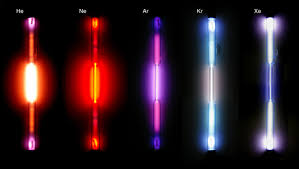
\includegraphics{gas_color.jpeg}

**

1859, Kirtchoff y Bunsen inventaron el espectroscopio y el siguiente año
por medio del análisis del espectro descubrieron dos elementos nuevos,
el cesio y el
rubidio***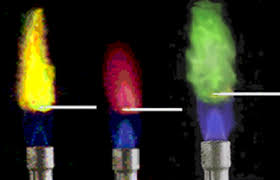
\includegraphics{elem2_color.jpeg}!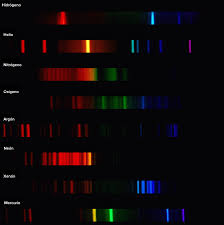
\includegraphics{elem_lineas.jpeg}

**

1885, Balmer encontró una expresión matemática para expresar las
longitudes de onda de las líneas observadas en el espectro del
hidrógeno**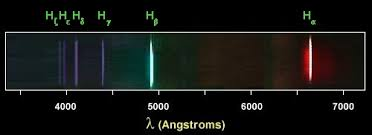
\includegraphics{lineas_Balmer.jpeg}

**

1897, J. J. Thomson demostró que los rayos catódicos eran partículas y
no ondas***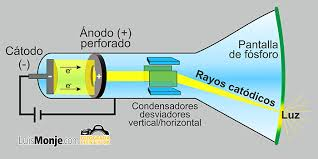
\includegraphics{ray_cathode.jpeg}

**

1897, Max Planck teniendo en cuenta los trabajos de Kirchoff, Wien,
Boltzmann y Stefan resolvó el misterio de la radiación del cuerpo
negro**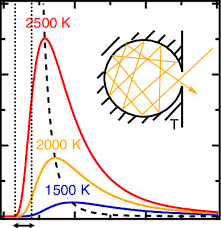
\includegraphics{black_body.png}

**

1905, Einstein, publicó tres trabajos en Annalen der Physik. En uno de
ellos desarrolló el concepto de cuantos de luz o fotones y explicó el
efecto fotoeléctrico.***\includegraphics{elec_effect.png}

**

1906 explicó la disminución del calor específico de los sólidos a medida
que se reduce la temperatura, suponiendo que los átomos de un cristal
tienen su energía cuantizada**

**

1911, Ernest Rutherford y Geiger y Marsden evidenciaron que los átomos
tienen un núcleo positivo con electrones negativos a su
alrededor***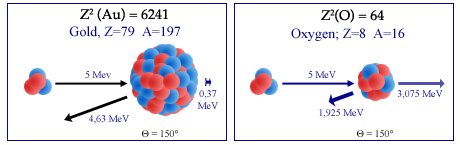
\includegraphics{Rutherford_En.jpg}

**

1913, Niel Bohr combinó el modelo atómico de Rutherford con la
revolucionaria teoría cuántica de Planck para diseñar la primera visión
matemática del átomo** 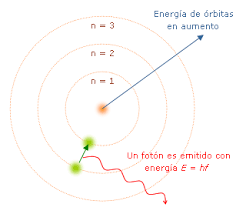
\includegraphics{at_bohr.png}

**

1923, Arthur Compton hizo medidas precisa de las colisión entre los
rayos X y los electrones, descubriendo que la longitud de los rayos X
aumenta.***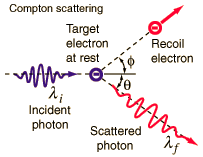
\includegraphics{ef_compton.png}

**

1924, Louis De Broglie desarrola la teoría que muestra la dualidad
onda-partícula, teorí que fue comprobada en 1927 por Davisson y Germer
en un experimento de difracción de electrones por un cristal de
níquel**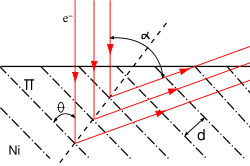
\includegraphics{Davisson_Germer.png}

    \begin{tcolorbox}[breakable, size=fbox, boxrule=1pt, pad at break*=1mm,colback=cellbackground, colframe=cellborder]
\prompt{In}{incolor}{1}{\boxspacing}
\begin{Verbatim}[commandchars=\\\{\}]
\PY{k+kn}{from} \PY{n+nn}{IPython}\PY{n+nn}{.}\PY{n+nn}{display} \PY{k+kn}{import} \PY{n}{HTML}
\end{Verbatim}
\end{tcolorbox}

    \begin{tcolorbox}[breakable, size=fbox, boxrule=1pt, pad at break*=1mm,colback=cellbackground, colframe=cellborder]
\prompt{In}{incolor}{2}{\boxspacing}
\begin{Verbatim}[commandchars=\\\{\}]
\PY{n}{HTML}\PY{p}{(}\PY{l+s+s1}{\PYZsq{}\PYZsq{}\PYZsq{}}\PY{l+s+s1}{\PYZlt{}script\PYZgt{}}
\PY{l+s+s1}{code\PYZus{}show=true; }
\PY{l+s+s1}{function code\PYZus{}toggle() }\PY{l+s+s1}{\PYZob{}}
\PY{l+s+s1}{ if (code\PYZus{}show)}\PY{l+s+s1}{\PYZob{}}
\PY{l+s+s1}{ \PYZdl{}(}\PY{l+s+s1}{\PYZsq{}}\PY{l+s+s1}{div.input}\PY{l+s+s1}{\PYZsq{}}\PY{l+s+s1}{).hide();}
\PY{l+s+s1}{ \PYZcb{} else }\PY{l+s+s1}{\PYZob{}}
\PY{l+s+s1}{ \PYZdl{}(}\PY{l+s+s1}{\PYZsq{}}\PY{l+s+s1}{div.input}\PY{l+s+s1}{\PYZsq{}}\PY{l+s+s1}{).show();}
\PY{l+s+s1}{ \PYZcb{}}
\PY{l+s+s1}{ code\PYZus{}show = !code\PYZus{}show}
\PY{l+s+s1}{\PYZcb{} }
\PY{l+s+s1}{\PYZdl{}( document ).ready(code\PYZus{}toggle);}
\PY{l+s+s1}{\PYZlt{}/script\PYZgt{}}
\PY{l+s+s1}{Los códigos de este }\PY{l+s+s1}{\PYZdq{}}\PY{l+s+s1}{IPython notebook}\PY{l+s+s1}{\PYZdq{}}\PY{l+s+s1}{ se mantienen ocultas por defecto para una mejor lectura. Las celdas aparecen vacias,}
\PY{l+s+s1}{con una línea azul en la parte izquierda, podrá observar los codigos en las celda haciendo click, \PYZlt{}a href=}\PY{l+s+s1}{\PYZdq{}}\PY{l+s+s1}{javascript:code\PYZus{}toggle()}\PY{l+s+s1}{\PYZdq{}}\PY{l+s+s1}{\PYZgt{}aquí\PYZlt{}/a\PYZgt{}.}\PY{l+s+s1}{\PYZsq{}\PYZsq{}\PYZsq{}}\PY{p}{)}
\end{Verbatim}
\end{tcolorbox}

            \begin{tcolorbox}[breakable, size=fbox, boxrule=.5pt, pad at break*=1mm, opacityfill=0]
\prompt{Out}{outcolor}{2}{\boxspacing}
\begin{Verbatim}[commandchars=\\\{\}]
<IPython.core.display.HTML object>
\end{Verbatim}
\end{tcolorbox}
        
    \begin{tcolorbox}[breakable, size=fbox, boxrule=1pt, pad at break*=1mm,colback=cellbackground, colframe=cellborder]
\prompt{In}{incolor}{3}{\boxspacing}
\begin{Verbatim}[commandchars=\\\{\}]
\PY{k+kn}{import} \PY{n+nn}{matplotlib} \PY{k}{as} \PY{n+nn}{mpl} \PY{c+c1}{\PYZsh{} matplotlib library for plotting and visualization}
\PY{k+kn}{import} \PY{n+nn}{matplotlib}\PY{n+nn}{.}\PY{n+nn}{pylab} \PY{k}{as} \PY{n+nn}{plt} \PY{c+c1}{\PYZsh{} matplotlib library for plotting and visualization}
\PY{k+kn}{import} \PY{n+nn}{numpy} \PY{k}{as} \PY{n+nn}{np} \PY{c+c1}{\PYZsh{}numpy library for numerical manipulation, especially suited for data arrays}
\PY{k+kn}{import} \PY{n+nn}{sympy} \PY{k}{as} \PY{n+nn}{sp}
\PY{c+c1}{\PYZsh{}from metakernel import register\PYZus{}ipython\PYZus{}magics}
\PY{c+c1}{\PYZsh{}register\PYZus{}ipython\PYZus{}magics()}
\end{Verbatim}
\end{tcolorbox}

    \begin{tcolorbox}[breakable, size=fbox, boxrule=1pt, pad at break*=1mm,colback=cellbackground, colframe=cellborder]
\prompt{In}{incolor}{4}{\boxspacing}
\begin{Verbatim}[commandchars=\\\{\}]
\PY{k+kn}{from} \PY{n+nn}{IPython}\PY{n+nn}{.}\PY{n+nn}{display} \PY{k+kn}{import} \PY{n}{Image}
\PY{n}{Image}\PY{p}{(}\PY{n}{filename}\PY{o}{=}\PY{l+s+s1}{\PYZsq{}}\PY{l+s+s1}{solvay\PYZus{}conference.jpg}\PY{l+s+s1}{\PYZsq{}}\PY{p}{,} \PY{n}{width}\PY{o}{=}\PY{l+m+mi}{700}\PY{p}{,} \PY{n}{height}\PY{o}{=}\PY{l+m+mi}{350}\PY{p}{)}
\end{Verbatim}
\end{tcolorbox}
 
            
\prompt{Out}{outcolor}{4}{}
    
    \begin{center}
    \adjustimage{max size={0.9\linewidth}{0.9\paperheight}}{output_6_0.jpg}
    \end{center}
    { \hspace*{\fill} \\}
    

    ¿Qué es la mecánica cuántica?

La mecánica cuántica es una teoría fundamental de la naturaleza que
describe las escalas más pequeñas y los niveles de energía de los átomos
y las partículas subatómicas.

\includegraphics{./content/images/qm.png}

\begin{itemize}
\item
  Las teorías cuánticas (incluyendo la mecánica cuántica y la teoría de
  campo cuántico) son teorías completas de nuestra realidad física que
  nunca han fallado desde su descubrimiento!
\item
  Las predicciones de la mecánica cuántica han sido verificadas
  experimentalmente con un grado de precisión extremadamente alto.
\end{itemize}

    ¿Dónde se aplica la Mecánica Cuántica

Las ideas de la mecánica cuántica están impregnadas y en muchos casos
constituyen la base de la comprensión de áreas enteras de la química, la
biología, la física y la ciencia de los materiales.

Algunos ejemplos son:

\hypertarget{enlace-quuxedmico-estructura-molecular-reactividad-color-propiedades-de-los-materiales.}{%
\subparagraph{\texorpdfstring{\textbf{Enlace químico, estructura
molecular, reactividad, color, propiedades de los
materiales.}}{Enlace químico, estructura molecular, reactividad, color, propiedades de los materiales.}}\label{enlace-quuxedmico-estructura-molecular-reactividad-color-propiedades-de-los-materiales.}}

\hypertarget{espectroscopia-rmn-uv-ir-luxe1ser}{%
\subparagraph{\texorpdfstring{\textbf{\emph{Espectroscopia (RMN, UV, IR,
láser\ldots{})}}}{Espectroscopia (RMN, UV, IR, láser\ldots{})}}\label{espectroscopia-rmn-uv-ir-luxe1ser}}

\hypertarget{cuxe1lculos-electruxf3nicos-modernos-de-estructura}{%
\subparagraph{\texorpdfstring{\textbf{Cálculos electrónicos modernos de
estructura}}{Cálculos electrónicos modernos de estructura}}\label{cuxe1lculos-electruxf3nicos-modernos-de-estructura}}

\hypertarget{materia-condensada}{%
\subparagraph{\texorpdfstring{\textbf{\emph{Materia
condensada}}}{Materia condensada}}\label{materia-condensada}}

\#\#\#\#\# \textbf{Computación cuántica}

    \begin{tcolorbox}[breakable, size=fbox, boxrule=1pt, pad at break*=1mm,colback=cellbackground, colframe=cellborder]
\prompt{In}{incolor}{5}{\boxspacing}
\begin{Verbatim}[commandchars=\\\{\}]
\PY{n}{Image}\PY{p}{(}\PY{n}{filename}\PY{o}{=}\PY{l+s+s1}{\PYZsq{}}\PY{l+s+s1}{Niels.jpeg}\PY{l+s+s1}{\PYZsq{}}\PY{p}{,} \PY{n}{width}\PY{o}{=}\PY{l+m+mi}{100}\PY{p}{,} \PY{n}{height}\PY{o}{=}\PY{l+m+mi}{100}\PY{p}{)}
\end{Verbatim}
\end{tcolorbox}
 
            
\prompt{Out}{outcolor}{5}{}
    
    \begin{center}
    \adjustimage{max size={0.9\linewidth}{0.9\paperheight}}{output_9_0.jpg}
    \end{center}
    { \hspace*{\fill} \\}
    

    \#\#\#

Niels Bohr: \textbf{\emph{``If you are not confused by quantum physics
then you haven't really understood it''}}

    \begin{tcolorbox}[breakable, size=fbox, boxrule=1pt, pad at break*=1mm,colback=cellbackground, colframe=cellborder]
\prompt{In}{incolor}{6}{\boxspacing}
\begin{Verbatim}[commandchars=\\\{\}]
\PY{n}{Image}\PY{p}{(}\PY{n}{filename}\PY{o}{=}\PY{l+s+s1}{\PYZsq{}}\PY{l+s+s1}{Feynman.jpeg}\PY{l+s+s1}{\PYZsq{}}\PY{p}{,} \PY{n}{width}\PY{o}{=}\PY{l+m+mi}{100}\PY{p}{,} \PY{n}{height}\PY{o}{=}\PY{l+m+mi}{100}\PY{p}{)}
\end{Verbatim}
\end{tcolorbox}
 
            
\prompt{Out}{outcolor}{6}{}
    
    \begin{center}
    \adjustimage{max size={0.9\linewidth}{0.9\paperheight}}{output_11_0.jpg}
    \end{center}
    { \hspace*{\fill} \\}
    

    \#\#\#

Richard Feynman: ''I think I can safely say that nobody understands
quantum mechanics''.

    **Charlas del Profesor Juan Carlos Paniagua sobre la sorprendente teoría
de la Mecánica Cuántica

    \begin{tcolorbox}[breakable, size=fbox, boxrule=1pt, pad at break*=1mm,colback=cellbackground, colframe=cellborder]
\prompt{In}{incolor}{7}{\boxspacing}
\begin{Verbatim}[commandchars=\\\{\}]
\PY{k+kn}{from} \PY{n+nn}{IPython}\PY{n+nn}{.}\PY{n+nn}{display} \PY{k+kn}{import} \PY{n}{YouTubeVideo}
\PY{n}{YouTubeVideo}\PY{p}{(}\PY{l+s+s1}{\PYZsq{}}\PY{l+s+s1}{N\PYZhy{}w1tkvdsQI}\PY{l+s+s1}{\PYZsq{}}\PY{p}{,} \PY{n}{width}\PY{o}{=}\PY{l+m+mi}{600}\PY{p}{,} \PY{n}{height}\PY{o}{=}\PY{l+m+mi}{300}\PY{p}{)}
\end{Verbatim}
\end{tcolorbox}
 
            
\prompt{Out}{outcolor}{7}{}
    
    \begin{center}
    \adjustimage{max size={0.9\linewidth}{0.9\paperheight}}{output_14_0.jpg}
    \end{center}
    { \hspace*{\fill} \\}
    

    \begin{tcolorbox}[breakable, size=fbox, boxrule=1pt, pad at break*=1mm,colback=cellbackground, colframe=cellborder]
\prompt{In}{incolor}{8}{\boxspacing}
\begin{Verbatim}[commandchars=\\\{\}]
\PY{k+kn}{from} \PY{n+nn}{IPython}\PY{n+nn}{.}\PY{n+nn}{display} \PY{k+kn}{import} \PY{n}{YouTubeVideo}
\PY{n}{YouTubeVideo}\PY{p}{(}\PY{l+s+s1}{\PYZsq{}}\PY{l+s+s1}{mS9ziEbMR\PYZus{}M}\PY{l+s+s1}{\PYZsq{}}\PY{p}{,} \PY{n}{width}\PY{o}{=}\PY{l+m+mi}{600}\PY{p}{,} \PY{n}{height}\PY{o}{=}\PY{l+m+mi}{300}\PY{p}{)}
\end{Verbatim}
\end{tcolorbox}
 
            
\prompt{Out}{outcolor}{8}{}
    
    \begin{center}
    \adjustimage{max size={0.9\linewidth}{0.9\paperheight}}{output_15_0.jpg}
    \end{center}
    { \hspace*{\fill} \\}
    

    \#

Postulados de Mecánica Cuántica

**

Un conjunto de postulados fundamentales hacen de la mecánica cuántica
una teoría lógica autocontenida. Armada con tal teoría, toda la química
y la biología ``en teoría'' se reduce a la mera aplicación de la
ecuación de Schrodinger. En la práctica la teoría no es tan fácil de
aplicar.**

**

El mundo microscópico tiene una naturaleza intrínsecamente
probabilística donde en algún sentido el mismo acto de observación crea
el resultado! La relación de incertidumbre pone un límite rígido a la
cantidad de información que uno puede poseer sobre los objetos
microscópicos.***

    \#\#

Postulado 1

    Todas las propiedades observables de un sistema físico están contenidas
en su función de onda, \(\Psi(q, t)\) , dependiente de las coordenadas
de posición \((q)\) de las partículas que componen el sistema, y del
tiempo \((t)\). Esta función debe ser univaluada, continúa, con
derivadas continúas, y de cuadrado integrable. \(|\Psi(q,t)|^2\) es, en
general, una función compleja, de modo que su cuadrado complejo es , se
interpreta como una densidad de probabilidad, de modo que expresa la
probabilidad de encontrar el sistema entre \(x\) y \(x+dx\) en un
instante de tiempo \(t\).

    \(\Psi(q,t)\) es, en general, una función compleja, de modo que su
cuadrado complejo \(|\Psi(q,t)|^2\), se interpreta como una densidad de
probabilidad, de modo que \(|\Psi(q,t)|^2dx\) expresa la probabilidad de
encontrar el sistema entre \(x\) y \(x+dx\) en un instante de tiempo
\(t\).

    \[\large \left<|\Psi(q,t)|^2dq\right>=\int^{+\infty}_{-\infty} |\Psi(q,t)|^2dq=1\]
si
\[\large \left<|\Psi(q,t)|^2dq\right>=\int^{+\infty}_{-\infty} |\Psi(q,t)|^2dq=b\]

\[\large \Psi(q,t)\Longrightarrow A\Psi(q,t)\] donde \(A\) se denomina
constante de Normalización y será igual a:
\[\large A=\frac{1}{\sqrt{b}}\]

    \#\#

Ejemplos

    **

Veamos estas funciones y verifiquemos el cumplimiento del postulado 1**

    \begin{tcolorbox}[breakable, size=fbox, boxrule=1pt, pad at break*=1mm,colback=cellbackground, colframe=cellborder]
\prompt{In}{incolor}{9}{\boxspacing}
\begin{Verbatim}[commandchars=\\\{\}]
\PY{k+kn}{from} \PY{n+nn}{matplotlib}\PY{n+nn}{.}\PY{n+nn}{font\PYZus{}manager} \PY{k+kn}{import} \PY{n}{FontProperties}
\PY{k+kn}{from} \PY{n+nn}{pylab} \PY{k+kn}{import} \PY{o}{*}

\PY{k}{def} \PY{n+nf}{f}\PY{p}{(}\PY{n}{t}\PY{p}{)}\PY{p}{:}
    \PY{n}{s1} \PY{o}{=} \PY{n}{cos}\PY{p}{(}\PY{l+m+mi}{2}\PY{o}{*}\PY{n}{pi}\PY{o}{*}\PY{n}{t}\PY{p}{)}
    \PY{n}{e1} \PY{o}{=} \PY{n}{exp}\PY{p}{(}\PY{o}{\PYZhy{}}\PY{n}{t}\PY{p}{)}
    \PY{k}{return} \PY{n}{multiply}\PY{p}{(}\PY{n}{s1}\PY{p}{,}\PY{n}{e1}\PY{p}{)}

\PY{n}{t1} \PY{o}{=} \PY{n}{arange}\PY{p}{(}\PY{l+m+mf}{0.0}\PY{p}{,} \PY{l+m+mf}{5.0}\PY{p}{,} \PY{l+m+mf}{0.1}\PY{p}{)}
\PY{n}{t2} \PY{o}{=} \PY{n}{arange}\PY{p}{(}\PY{l+m+mf}{0.0}\PY{p}{,} \PY{l+m+mf}{5.0}\PY{p}{,} \PY{l+m+mf}{0.02}\PY{p}{)}
\PY{n}{t3} \PY{o}{=} \PY{n}{arange}\PY{p}{(}\PY{l+m+mf}{0.0}\PY{p}{,} \PY{l+m+mf}{2.0}\PY{p}{,} \PY{l+m+mf}{0.01}\PY{p}{)}


\PY{n}{subplot}\PY{p}{(}\PY{l+m+mi}{151}\PY{p}{)}
\PY{n}{plot}\PY{p}{(}\PY{n}{t1}\PY{p}{,} \PY{n}{f}\PY{p}{(}\PY{n}{t1}\PY{p}{)}\PY{p}{,} \PY{l+s+s1}{\PYZsq{}}\PY{l+s+s1}{bo}\PY{l+s+s1}{\PYZsq{}}\PY{p}{,} \PY{n}{t2}\PY{p}{,} \PY{n}{f}\PY{p}{(}\PY{n}{t2}\PY{p}{)}\PY{p}{,} \PY{l+s+s1}{\PYZsq{}}\PY{l+s+s1}{k}\PY{l+s+s1}{\PYZsq{}}\PY{p}{,} \PY{n}{linewidth}\PY{o}{=}\PY{l+m+mi}{5}\PY{p}{)}
\PY{n}{title}\PY{p}{(}\PY{l+s+s1}{\PYZsq{}}\PY{l+s+s1}{\PYZdl{}f(x)=e\PYZca{}}\PY{l+s+s1}{\PYZob{}}\PY{l+s+s1}{\PYZhy{}t\PYZcb{}cos(2 }\PY{l+s+s1}{\PYZbs{}}\PY{l+s+s1}{pi t)\PYZdl{}}\PY{l+s+s1}{\PYZsq{}}\PY{p}{,} \PY{n}{fontsize}\PY{o}{=}\PY{l+m+mi}{35}\PY{p}{)}


\PY{n}{subplot}\PY{p}{(}\PY{l+m+mi}{152}\PY{p}{)}
\PY{n}{plot}\PY{p}{(}\PY{n}{t3}\PY{p}{,} \PY{n}{cos}\PY{p}{(}\PY{l+m+mi}{2}\PY{o}{*}\PY{n}{pi}\PY{o}{*}\PY{n}{t3}\PY{p}{)}\PY{p}{,} \PY{l+s+s1}{\PYZsq{}}\PY{l+s+s1}{r\PYZhy{}\PYZhy{}}\PY{l+s+s1}{\PYZsq{}}\PY{p}{,} \PY{n}{linewidth}\PY{o}{=}\PY{l+m+mi}{3}\PY{p}{)}
\PY{n}{xlabel}\PY{p}{(}\PY{l+s+s1}{\PYZsq{}}\PY{l+s+s1}{tiempo (s)}\PY{l+s+s1}{\PYZsq{}}\PY{p}{)}
\PY{n}{title}\PY{p}{(}\PY{l+s+s1}{\PYZsq{}}\PY{l+s+s1}{\PYZdl{}f(x)=cos(2 }\PY{l+s+s1}{\PYZbs{}}\PY{l+s+s1}{pi t)\PYZdl{}}\PY{l+s+s1}{\PYZsq{}}\PY{p}{,} \PY{n}{fontsize}\PY{o}{=}\PY{l+m+mi}{35}\PY{p}{)}


\PY{n}{subplot}\PY{p}{(}\PY{l+m+mi}{153}\PY{p}{)}
\PY{n}{plot}\PY{p}{(}\PY{n}{t3}\PY{p}{,} \PY{n}{exp}\PY{p}{(}\PY{o}{\PYZhy{}}\PY{n}{t3}\PY{p}{)}\PY{p}{,} \PY{l+s+s1}{\PYZsq{}}\PY{l+s+s1}{g\PYZhy{}}\PY{l+s+s1}{\PYZsq{}}\PY{p}{,} \PY{n}{linewidth}\PY{o}{=}\PY{l+m+mi}{3}\PY{p}{)}
\PY{n}{title}\PY{p}{(}\PY{l+s+s1}{\PYZsq{}}\PY{l+s+s1}{\PYZdl{}f(x)=e\PYZca{}}\PY{l+s+s1}{\PYZob{}}\PY{l+s+s1}{\PYZhy{}t\PYZcb{}\PYZdl{}}\PY{l+s+s1}{\PYZsq{}}\PY{p}{,} \PY{n}{fontsize}\PY{o}{=}\PY{l+m+mi}{35}\PY{p}{)}


\PY{k}{with} \PY{n}{plt}\PY{o}{.}\PY{n}{xkcd}\PY{p}{(}\PY{p}{)}\PY{p}{:}
    \PY{n}{subplot}\PY{p}{(}\PY{l+m+mi}{154}\PY{p}{)}
    \PY{n}{x} \PY{o}{=} \PY{n}{np}\PY{o}{.}\PY{n}{linspace}\PY{p}{(}\PY{l+m+mi}{0}\PY{p}{,} \PY{l+m+mi}{10}\PY{p}{)}
    \PY{n}{line}\PY{p}{,} \PY{o}{=} \PY{n}{plt}\PY{o}{.}\PY{n}{plot}\PY{p}{(}\PY{n}{x}\PY{p}{,} \PY{n}{np}\PY{o}{.}\PY{n}{sin}\PY{p}{(}\PY{n}{x}\PY{o}{*}\PY{n}{pi}\PY{p}{)}\PY{p}{,} \PY{l+s+s1}{\PYZsq{}}\PY{l+s+s1}{b\PYZhy{}}\PY{l+s+s1}{\PYZsq{}}\PY{p}{,} \PY{n}{linewidth}\PY{o}{=}\PY{l+m+mi}{5}\PY{p}{)}
\PY{n}{title}\PY{p}{(}\PY{l+s+s1}{\PYZsq{}}\PY{l+s+s1}{\PYZdl{}f(x)=sen(x)\PYZdl{}}\PY{l+s+s1}{\PYZsq{}}\PY{p}{,} \PY{n}{fontsize}\PY{o}{=}\PY{l+m+mi}{35}\PY{p}{)}


\PY{n}{subplot}\PY{p}{(}\PY{l+m+mi}{155}\PY{p}{)}
\PY{n}{x} \PY{o}{=} \PY{n}{np}\PY{o}{.}\PY{n}{linspace}\PY{p}{(}\PY{o}{\PYZhy{}}\PY{l+m+mi}{10}\PY{p}{,} \PY{l+m+mi}{10}\PY{p}{)}
\PY{n}{line}\PY{p}{,} \PY{o}{=} \PY{n}{plt}\PY{o}{.}\PY{n}{plot}\PY{p}{(}\PY{n}{x}\PY{p}{,} \PY{n}{np}\PY{o}{.}\PY{n}{abs}\PY{p}{(}\PY{n}{x}\PY{p}{)}\PY{p}{,} \PY{l+s+s1}{\PYZsq{}}\PY{l+s+s1}{r\PYZhy{}}\PY{l+s+s1}{\PYZsq{}}\PY{p}{,} \PY{n}{linewidth}\PY{o}{=}\PY{l+m+mi}{3}\PY{p}{)}
\PY{n}{title}\PY{p}{(}\PY{l+s+s1}{\PYZsq{}}\PY{l+s+s1}{\PYZdl{}f(x)=|x|\PYZdl{}}\PY{l+s+s1}{\PYZsq{}}\PY{p}{,} \PY{n}{fontsize}\PY{o}{=}\PY{l+m+mi}{35}\PY{p}{)}
\PY{n}{plt}\PY{o}{.}\PY{n}{subplots\PYZus{}adjust}\PY{p}{(}\PY{n}{wspace}\PY{o}{=}\PY{l+m+mf}{0.1}\PY{p}{,} \PY{n}{hspace}\PY{o}{=}\PY{l+m+mf}{0.1}\PY{p}{,} \PY{n}{top}\PY{o}{=}\PY{l+m+mf}{1.5}\PY{p}{,} \PY{n}{right}\PY{o}{=}\PY{l+m+mi}{5}\PY{p}{)}
\PY{n}{show}\PY{p}{(}\PY{p}{)}
\end{Verbatim}
\end{tcolorbox}

    \begin{Verbatim}[commandchars=\\\{\}]
<>:16: DeprecationWarning: invalid escape sequence \textbackslash{}p
<>:22: DeprecationWarning: invalid escape sequence \textbackslash{}p
<>:16: DeprecationWarning: invalid escape sequence \textbackslash{}p
<>:22: DeprecationWarning: invalid escape sequence \textbackslash{}p
<ipython-input-9-0d697cec178f>:16: DeprecationWarning: invalid escape sequence
\textbackslash{}p
  title('\$f(x)=e\^{}\{-t\}cos(2 \textbackslash{}pi t)\$', fontsize=35)
<ipython-input-9-0d697cec178f>:22: DeprecationWarning: invalid escape sequence
\textbackslash{}p
  title('\$f(x)=cos(2 \textbackslash{}pi t)\$', fontsize=35)
findfont: Font family ['xkcd', 'xkcd Script', 'Humor Sans', 'Comic Neue', 'Comic
Sans MS'] not found. Falling back to DejaVu Sans.
findfont: Font family ['xkcd', 'xkcd Script', 'Humor Sans', 'Comic Neue', 'Comic
Sans MS'] not found. Falling back to DejaVu Sans.
findfont: Font family ['xkcd', 'xkcd Script', 'Humor Sans', 'Comic Neue', 'Comic
Sans MS'] not found. Falling back to DejaVu Sans.
    \end{Verbatim}

    \begin{center}
    \adjustimage{max size={0.9\linewidth}{0.9\paperheight}}{output_23_1.png}
    \end{center}
    { \hspace*{\fill} \\}
    
    \begin{tcolorbox}[breakable, size=fbox, boxrule=1pt, pad at break*=1mm,colback=cellbackground, colframe=cellborder]
\prompt{In}{incolor}{10}{\boxspacing}
\begin{Verbatim}[commandchars=\\\{\}]
\PY{k+kn}{import} \PY{n+nn}{numpy} \PY{k}{as} \PY{n+nn}{np}
\PY{k+kn}{import} \PY{n+nn}{pylab} \PY{k}{as} \PY{n+nn}{pl}
\PY{k+kn}{from} \PY{n+nn}{scipy} \PY{k+kn}{import} \PY{n}{interpolate}\PY{p}{,} \PY{n}{signal}
\PY{k+kn}{import} \PY{n+nn}{matplotlib}\PY{n+nn}{.}\PY{n+nn}{font\PYZus{}manager} \PY{k}{as} \PY{n+nn}{fm}
\end{Verbatim}
\end{tcolorbox}

    \#\#\#\#

Veamos si las funciones son derivables (contínuas) \[f(x)=e^{-x}cos(x)\]
\[\frac{df(x)}{dx}= −𝑒^{-𝑥}sin(𝑥)−𝑒^{-𝑥}cos(𝑥)\]

    \begin{tcolorbox}[breakable, size=fbox, boxrule=1pt, pad at break*=1mm,colback=cellbackground, colframe=cellborder]
\prompt{In}{incolor}{11}{\boxspacing}
\begin{Verbatim}[commandchars=\\\{\}]
\PY{n}{x} \PY{o}{=} \PY{n}{sp}\PY{o}{.}\PY{n}{Symbol}\PY{p}{(}\PY{l+s+s1}{\PYZsq{}}\PY{l+s+s1}{x}\PY{l+s+s1}{\PYZsq{}}\PY{p}{)} 
\PY{n}{y} \PY{o}{=} \PY{n}{sp}\PY{o}{.}\PY{n}{cos}\PY{p}{(}\PY{n}{x}\PY{p}{)}\PY{o}{*}\PY{n}{sp}\PY{o}{.}\PY{n}{exp}\PY{p}{(}\PY{o}{\PYZhy{}}\PY{n}{x}\PY{p}{)} 
\PY{n}{sp}\PY{o}{.}\PY{n}{diff}\PY{p}{(}\PY{n}{y}\PY{p}{,}\PY{n}{x}\PY{p}{)}
\end{Verbatim}
\end{tcolorbox}
 
            
\prompt{Out}{outcolor}{11}{}
    
    $\displaystyle - e^{- x} \sin{\left(x \right)} - e^{- x} \cos{\left(x \right)}$

    

    \[\large f(x)=cos(x)\] \[\large \frac{f(x)}{dx}= −sin(𝑥)\]

    \begin{tcolorbox}[breakable, size=fbox, boxrule=1pt, pad at break*=1mm,colback=cellbackground, colframe=cellborder]
\prompt{In}{incolor}{12}{\boxspacing}
\begin{Verbatim}[commandchars=\\\{\}]
\PY{n}{x} \PY{o}{=} \PY{n}{sp}\PY{o}{.}\PY{n}{Symbol}\PY{p}{(}\PY{l+s+s1}{\PYZsq{}}\PY{l+s+s1}{x}\PY{l+s+s1}{\PYZsq{}}\PY{p}{)} 
\PY{n}{y} \PY{o}{=} \PY{n}{sp}\PY{o}{.}\PY{n}{cos}\PY{p}{(}\PY{n}{x}\PY{p}{)} 
\PY{n}{sp}\PY{o}{.}\PY{n}{diff}\PY{p}{(}\PY{n}{y}\PY{p}{,}\PY{n}{x}\PY{p}{)}
\end{Verbatim}
\end{tcolorbox}
 
            
\prompt{Out}{outcolor}{12}{}
    
    $\displaystyle - \sin{\left(x \right)}$

    

    \[\large f(x)=e^{-x}\] \[\large \frac{df(x)}{dx}= −𝑒^{-𝑥}\]

    \begin{tcolorbox}[breakable, size=fbox, boxrule=1pt, pad at break*=1mm,colback=cellbackground, colframe=cellborder]
\prompt{In}{incolor}{13}{\boxspacing}
\begin{Verbatim}[commandchars=\\\{\}]
\PY{n}{x} \PY{o}{=} \PY{n}{sp}\PY{o}{.}\PY{n}{Symbol}\PY{p}{(}\PY{l+s+s1}{\PYZsq{}}\PY{l+s+s1}{x}\PY{l+s+s1}{\PYZsq{}}\PY{p}{)} 
\PY{n}{y} \PY{o}{=} \PY{n}{sp}\PY{o}{.}\PY{n}{exp}\PY{p}{(}\PY{o}{\PYZhy{}}\PY{n}{x}\PY{p}{)} 
\PY{n}{sp}\PY{o}{.}\PY{n}{diff}\PY{p}{(}\PY{n}{y}\PY{p}{,}\PY{n}{x}\PY{p}{)}
\end{Verbatim}
\end{tcolorbox}
 
            
\prompt{Out}{outcolor}{13}{}
    
    $\displaystyle - e^{- x}$

    

    \[\large f(x)= |x|\] \[\large \frac{df(x)}{dx}= Indeter\]

    \begin{tcolorbox}[breakable, size=fbox, boxrule=1pt, pad at break*=1mm,colback=cellbackground, colframe=cellborder]
\prompt{In}{incolor}{14}{\boxspacing}
\begin{Verbatim}[commandchars=\\\{\}]
\PY{n}{x} \PY{o}{=} \PY{n}{sp}\PY{o}{.}\PY{n}{Symbol}\PY{p}{(}\PY{l+s+s1}{\PYZsq{}}\PY{l+s+s1}{x}\PY{l+s+s1}{\PYZsq{}}\PY{p}{)} 
\PY{n}{y} \PY{o}{=} \PY{n}{np}\PY{o}{.}\PY{n}{abs}\PY{p}{(}\PY{n}{x}\PY{p}{)} 
\PY{n}{sp}\PY{o}{.}\PY{n}{diff}\PY{p}{(}\PY{n}{y}\PY{p}{,}\PY{n}{x}\PY{p}{)}
\end{Verbatim}
\end{tcolorbox}
 
            
\prompt{Out}{outcolor}{14}{}
    
    $\displaystyle \frac{\left(\operatorname{re}{\left(x\right)} \frac{d}{d x} \operatorname{re}{\left(x\right)} + \operatorname{im}{\left(x\right)} \frac{d}{d x} \operatorname{im}{\left(x\right)}\right) \operatorname{sign}{\left(x \right)}}{x}$

    

    \#\#\#

Segunda derivada**

\[\large f(x)=e^{-x}cos(x)\]
\[\large \frac{d^2f(x)}{dx^2}= 2e^{-x}sen(𝑥)\]

    \begin{tcolorbox}[breakable, size=fbox, boxrule=1pt, pad at break*=1mm,colback=cellbackground, colframe=cellborder]
\prompt{In}{incolor}{15}{\boxspacing}
\begin{Verbatim}[commandchars=\\\{\}]
\PY{n}{x} \PY{o}{=} \PY{n}{sp}\PY{o}{.}\PY{n}{Symbol}\PY{p}{(}\PY{l+s+s1}{\PYZsq{}}\PY{l+s+s1}{x}\PY{l+s+s1}{\PYZsq{}}\PY{p}{)} 
\PY{n}{y} \PY{o}{=} \PY{n}{sp}\PY{o}{.}\PY{n}{cos}\PY{p}{(}\PY{n}{x}\PY{p}{)}\PY{o}{*}\PY{n}{sp}\PY{o}{.}\PY{n}{exp}\PY{p}{(}\PY{o}{\PYZhy{}}\PY{n}{x}\PY{p}{)} 
\PY{n}{sp}\PY{o}{.}\PY{n}{diff}\PY{p}{(}\PY{n}{y}\PY{p}{,}\PY{n}{x}\PY{p}{,}\PY{l+m+mi}{2}\PY{p}{)}
\end{Verbatim}
\end{tcolorbox}
 
            
\prompt{Out}{outcolor}{15}{}
    
    $\displaystyle 2 e^{- x} \sin{\left(x \right)}$

    

    \[\large f(x)=e^{-x}\] \[\large \frac{d^2f(x)}{dx^2}= e^{-x}\]

    \begin{tcolorbox}[breakable, size=fbox, boxrule=1pt, pad at break*=1mm,colback=cellbackground, colframe=cellborder]
\prompt{In}{incolor}{16}{\boxspacing}
\begin{Verbatim}[commandchars=\\\{\}]
\PY{n}{x} \PY{o}{=} \PY{n}{sp}\PY{o}{.}\PY{n}{Symbol}\PY{p}{(}\PY{l+s+s1}{\PYZsq{}}\PY{l+s+s1}{x}\PY{l+s+s1}{\PYZsq{}}\PY{p}{)} 
\PY{n}{y} \PY{o}{=} \PY{n}{sp}\PY{o}{.}\PY{n}{exp}\PY{p}{(}\PY{o}{\PYZhy{}}\PY{n}{x}\PY{p}{)} 
\PY{n}{sp}\PY{o}{.}\PY{n}{diff}\PY{p}{(}\PY{n}{y}\PY{p}{,}\PY{n}{x}\PY{p}{,}\PY{l+m+mi}{2}\PY{p}{)}
\end{Verbatim}
\end{tcolorbox}
 
            
\prompt{Out}{outcolor}{16}{}
    
    $\displaystyle e^{- x}$

    

    \[\large f(x)=e^{-x}cos(x)\] \[\large \frac{d^2f(x)}{dx^2}= −cos(𝑥)\]

    \begin{tcolorbox}[breakable, size=fbox, boxrule=1pt, pad at break*=1mm,colback=cellbackground, colframe=cellborder]
\prompt{In}{incolor}{17}{\boxspacing}
\begin{Verbatim}[commandchars=\\\{\}]
\PY{n}{x} \PY{o}{=} \PY{n}{sp}\PY{o}{.}\PY{n}{Symbol}\PY{p}{(}\PY{l+s+s1}{\PYZsq{}}\PY{l+s+s1}{x}\PY{l+s+s1}{\PYZsq{}}\PY{p}{)} 
\PY{n}{y} \PY{o}{=} \PY{n}{sp}\PY{o}{.}\PY{n}{cos}\PY{p}{(}\PY{n}{x}\PY{p}{)} 
\PY{n}{sp}\PY{o}{.}\PY{n}{diff}\PY{p}{(}\PY{n}{y}\PY{p}{,}\PY{n}{x}\PY{p}{,}\PY{l+m+mi}{2}\PY{p}{)}
\end{Verbatim}
\end{tcolorbox}
 
            
\prompt{Out}{outcolor}{17}{}
    
    $\displaystyle - \cos{\left(x \right)}$

    

    \#\#\#

Cuadrado integrable \(\left<|\Psi(q,t)|^2dq\right>=b\), donde \(b\) es
un número finito

\[\large \int^{2\pi}_{0} |e^{-x}cos(x)|^2dx=\frac{3}{8}-\frac{3}{8e^{4\pi}}\]

    \begin{tcolorbox}[breakable, size=fbox, boxrule=1pt, pad at break*=1mm,colback=cellbackground, colframe=cellborder]
\prompt{In}{incolor}{18}{\boxspacing}
\begin{Verbatim}[commandchars=\\\{\}]
\PY{c+c1}{\PYZsh{}Integral definidas entre 0 e infinito}
\PY{c+c1}{\PYZsh{}from \PYZus{}\PYZus{}future\PYZus{}\PYZus{} import division}
\PY{k+kn}{from} \PY{n+nn}{sympy} \PY{k+kn}{import} \PY{o}{*}
\PY{n}{x}\PY{p}{,} \PY{n}{y}\PY{p}{,} \PY{n}{z}\PY{p}{,} \PY{n}{t} \PY{o}{=} \PY{n}{symbols}\PY{p}{(}\PY{l+s+s1}{\PYZsq{}}\PY{l+s+s1}{x y z t}\PY{l+s+s1}{\PYZsq{}}\PY{p}{)}
\PY{n}{k}\PY{p}{,} \PY{n}{m}\PY{p}{,} \PY{n}{n} \PY{o}{=} \PY{n}{symbols}\PY{p}{(}\PY{l+s+s1}{\PYZsq{}}\PY{l+s+s1}{k m n}\PY{l+s+s1}{\PYZsq{}}\PY{p}{,} \PY{n}{integer}\PY{o}{=}\PY{k+kc}{True}\PY{p}{)}
\PY{n}{f}\PY{p}{,} \PY{n}{g}\PY{p}{,} \PY{n}{h} \PY{o}{=} \PY{n}{symbols}\PY{p}{(}\PY{l+s+s1}{\PYZsq{}}\PY{l+s+s1}{f g h}\PY{l+s+s1}{\PYZsq{}}\PY{p}{,} \PY{n+nb+bp}{cls}\PY{o}{=}\PY{n}{Function}\PY{p}{)}

\PY{n}{sp}\PY{o}{.}\PY{n}{integrate}\PY{p}{(}\PY{p}{(}\PY{n}{sp}\PY{o}{.}\PY{n}{exp}\PY{p}{(}\PY{o}{\PYZhy{}}\PY{n}{x}\PY{p}{)}\PY{o}{*}\PY{n}{sp}\PY{o}{.}\PY{n}{cos}\PY{p}{(}\PY{n}{x}\PY{p}{)}\PY{p}{)}\PY{o}{*}\PY{o}{*}\PY{l+m+mi}{2}\PY{p}{,} \PY{p}{(}\PY{n}{x}\PY{p}{,} \PY{l+m+mi}{0}\PY{p}{,} \PY{l+m+mi}{2}\PY{o}{*}\PY{n}{sp}\PY{o}{.}\PY{n}{pi}\PY{p}{)}\PY{p}{)}
\end{Verbatim}
\end{tcolorbox}
 
            
\prompt{Out}{outcolor}{18}{}
    
    $\displaystyle \frac{3}{8} - \frac{3}{8 e^{4 \pi}}$

    

    \[\large \int^{2\pi}_{0} |e^{-x}|^2dx=\frac{1}{2}-\frac{1}{2e^{4\pi}}\]

    \begin{tcolorbox}[breakable, size=fbox, boxrule=1pt, pad at break*=1mm,colback=cellbackground, colframe=cellborder]
\prompt{In}{incolor}{19}{\boxspacing}
\begin{Verbatim}[commandchars=\\\{\}]
\PY{n}{sp}\PY{o}{.}\PY{n}{integrate}\PY{p}{(}\PY{p}{(}\PY{n}{sp}\PY{o}{.}\PY{n}{exp}\PY{p}{(}\PY{o}{\PYZhy{}}\PY{n}{x}\PY{p}{)}\PY{p}{)}\PY{o}{*}\PY{o}{*}\PY{l+m+mi}{2}\PY{p}{,} \PY{p}{(}\PY{n}{x}\PY{p}{,} \PY{l+m+mi}{0}\PY{p}{,} \PY{l+m+mi}{2}\PY{o}{*}\PY{n}{sp}\PY{o}{.}\PY{n}{pi}\PY{p}{)}\PY{p}{)}
\end{Verbatim}
\end{tcolorbox}
 
            
\prompt{Out}{outcolor}{19}{}
    
    $\displaystyle \frac{1}{2} - \frac{1}{2 e^{4 \pi}}$

    

    \[\large \int^{2\pi}_{0} |cos(x)|^2dx=\pi\]

    \begin{tcolorbox}[breakable, size=fbox, boxrule=1pt, pad at break*=1mm,colback=cellbackground, colframe=cellborder]
\prompt{In}{incolor}{20}{\boxspacing}
\begin{Verbatim}[commandchars=\\\{\}]
\PY{n}{sp}\PY{o}{.}\PY{n}{integrate}\PY{p}{(}\PY{p}{(}\PY{p}{(}\PY{n}{sp}\PY{o}{.}\PY{n}{cos}\PY{p}{(}\PY{n}{x}\PY{p}{)}\PY{p}{)}\PY{o}{*}\PY{o}{*}\PY{l+m+mi}{2}\PY{p}{)}\PY{p}{,} \PY{p}{(}\PY{n}{x}\PY{p}{,} \PY{l+m+mi}{0}\PY{p}{,} \PY{l+m+mi}{2}\PY{o}{*}\PY{n}{sp}\PY{o}{.}\PY{n}{pi}\PY{p}{)}\PY{p}{)}
\end{Verbatim}
\end{tcolorbox}
 
            
\prompt{Out}{outcolor}{20}{}
    
    $\displaystyle \pi$

    

    \#\#

Postulado 2

    Sean dos funciones de onda cualesquiera, \(\Psi_1(q, t)\) y
\(\Psi_2(q, t)\), que representan estados de un mismo sistema, y sean
dos números complejos arbitrarios \(c_1\) y \(c_2\). La combinación
lineal es la función de onda de un estado valido
\(\Psi(q,t)=c_1\Psi_1(q, t)+c_2\Psi_2(q, t)\) del sistema, y este estado
se dice que es una superposición de los estados representados por
\(\Psi_1(q, t)\) y \(\Psi_2(q, t)\).

La probabilidad del estado superpuesto no es una simple suma de las
probabilidades de los estados que se superponen. De otro modo, las
funciones de onda se suman pero la información está contenida en su
cuadrado. Esta regla permite explicar los fenómenos ondulatorios, tales
como la difracción de electrones o neutrones.

    \#\#\#\#

Espacios de Hilbert

    La colección de todas las funciones de x constituye un espacio de
vectores. Pero para representar un estado físico posible, deben
normalizarse las funciones de onda:

     \[\large \int^{+\infty}_{-\infty} |\Psi(q,t)|^2dq=1\]

    \#\#\#\#\#

Normalización, ortogonalidad

     \[\large \int^{+\infty}_{-\infty} |f*(q,t)f(q,t)|dq=1\] entonces
\(f(q,t)\) están normalizada

     \[\large \int^{+\infty}_{-\infty} |f^*(q,t)g(q,t)|dq=0\] entonces
\(f(q,t)\) y \(g(q,t)\) son ortogonales

    Si un conjunto de funciones, \(f(n)\), es ortonormal si están
normalizadas y son mutuamente ortogonales:

     \[\large \int^{+\infty}_{-\infty} f^*_{m}g_{n}d\tau=\delta_{mn}\]

     \[\large \left<f^*_{m}|g_{n}\right>=\delta_{mn}\]

    \#\#

Postulado 3

    Cada observable físico, L, se representa mediante un operador lineal y
hermítico \(\hat L\), La linealidad de los opeartores se desprende de la
naturaleza de la ecuación de Schrodinger, que es una ecuación
diferencial lineal. La linealidad implica una propiedad distirbutiva de
los opeartores cuando se aplica a cualquier combinación lineal de
funciones.

\[\hat{L} (c_1\psi_1+c_2\psi_2+...+c_n\psi_n)=c_1\hat{L} \psi_1+c_2\hat{L}\psi_2+...+c_n\hat{L}\psi_n \]

De otro lado, La propiedad hermiticidad de los operadores garantiza que
los valores propios son estrictamente reales. Y como los valores propios
son los únicos valores observados en las mediciones experimentales, es
razonable esperar que no se mezclen números complejos y reales en los
experimentos. la propiedad de hermiticidad se define por la siguiente
igualdad, en la que un operador puede entrar en modo de conjugado
complejo y actuar sobre el par conjugado complejo de la función.

\[\int \psi^* (\hat{H} \phi) dx = \int \phi (\hat{H} \psi)^* dx =\int \phi \hat{H}^* \psi^* dx \]

    \#\#\#

Operadores mecánico-cuánticos

Gracias a la universalidad de la ley de conservación de la energía, por
cada observable en la mecánica clásica se puede encontrar un operador
correspondiente en la mecánica cuántica! El {operador posición} se
describe en en la dirección \(x\), \(\hat{x}=x\), siendo un operador de
carácter multiplicativoy que se puede exteneder a las tres dimensiones
como
\(\large \hat{\vec r}= \hat{x}\vec i + \hat{y}\vec j + \hat{z}\vec k\).
{Operador Momento Lineal}, 1D:
\[\large \hat{p_x}=\frac{\hbar}{i}\frac{d}{dx}\] 3D:
\[\large \hat{p}_{3D}=\frac{\hbar}{i}[\frac{\partial}{\partial x}\vec i + \frac{\partial}{\partial y}\vec j + \frac{\partial}{\partial z}\vec k]\]
{Operador Energía Cinética}, \(\hat T\) , clásicamente se define como
\[\large T=\frac{p^2}{2m}\] entonces el operador en 1D:
\[\large \hat{T_x}=-\frac{\hbar^2}{2m}\frac{d^2}{dx^2}\] 3D:
\[\large \hat{T}_{3D}=-\frac{\hbar^2}{2m}[\frac{\partial^2}{\partial x^2}\vec i + \frac{\partial^2}{\partial y^2}\vec j + \frac{\partial^2}{\partial z^2}\vec k]\]
{Operador Energía Potencial}, \[\large \hat{V}=V(x)\] {Operador Momento
Angular}a partir del término clásico,
\(\large \vec{L}=\vec r x \vec p\), de aquí construímos el operador
mecánico-cuántico
\[\large \hat{L}=\begin{bmatrix} \vec i &\vec j &\vec k \\ \hat x &\hat y &\hat z \\ \hat{p}_x &\hat{p}_y &\hat{p}_z\end{bmatrix}\]
{Operador Energía Total, Hamiltoniano}
\(\Longrightarrow \large \hat{H}=\hat{T}+\hat{V}\)
\[\large \hat{H}=-\frac{\hbar^2}{2m}[\frac{\partial^2}{\partial x^2}\vec i + \frac{\partial^2}{\partial y^2}\vec j + \frac{\partial^2}{\partial z^2}\vec k] + \hat V(x,y,z)\]
\[\large \hat{H}=-\frac{\hbar^2}{2m}\hat{\vec{\nabla}}^2 + \hat V(x,y,z)\]

    \#\#\#

Conmutación de los Operadores

Dos operadores \(\hat A\) y \(\hat B\) conmutan si cumplen \$
{[}\hat{A},\hat{B}{]}=\hat{AB} - \hat{BA}=0 \$, la conmutación de dos
operadores ímplica que que es posible determinar de forma simultánea y
precisa los valores de la variable física que ellos representan.

Como ejemplo:

\[ \large [\hat{x},\hat{p_x}] = \hat{x{p_x}}-\hat{{p_x}x}=i\hbar\]

En general:

\[ \large [\hat{\xi},\hat{p_{\zeta}}]=i\hbar \hat{p}_{\xi \zeta}, [\hat{\xi},\hat{\zeta}]=0, [\hat{p}_{\xi},\hat{p}_{\zeta}]=0 \]
donde \(\large \xi, \zeta = x,y,z\)

    \#\#

Postulado 4

    Una medida única, individual, de la propiedad fìsica (observable)
asociada al operador \(\hat{A}\) debe dar como resultado uno de los
valores propios del operador. Decimos que \(\Psi_n\) es una función
propia del operador \(\hat{A}\), con valor propio \(a_n\) si
\[\large \hat{A}\Psi_{n}=a_n\Psi_{n}\] {Esta ecuaciòn se denomina
ecuación de valor propio}

    \#\#

Postulado 5

    Sea \(\Psi_{n}\) una función propia arbitraria de \(\hat{A}\):
\(\hat{A}\Psi_{n}= a_n\Psi_{n}\). El conjunto de todas las funciones
propias independientes forma un conjunto completo, de modo que la
función de onda de un estado cualesquiera del sistema se puede escribir
siempre como una combinación lineal de las funciones propias
independientes: \[\large \Psi(q,t)=\sum_{n} C_{n}\Psi_{n}(q,t)\]

    \#\#

Postulado 6

    Si la función de onda y el operador asociado a un observable no cumplen
con {la ecuación de valor propio}, entonces la medición del observable
asociado al operador \(\hat{A}\) en un estado
mezcla,\(\Psi(q,t)=\sum_{n} C_{n}\Psi_{n}(q,t)\) transforma el estado
del sistema al estado propio \(\Psi_{n}\) y da como resultado el valor
propio \(a_n\) con una probabilidad proporcional a \(|c_n|^2\). En
consecuencia, el valor promedio de una colección de medidas de
\(\hat{A}\) es

\[\large \left<A\right>=\frac{\int^{+\infty}_{-\infty} \Psi^* \hat{A}\Psi d\tau}{\int^{+\infty}_{-\infty} |\Psi|^2d\tau}\]

    \#\#

Postulado 7

    En 1925/1926 Erwin Schrodinger, que era un experto en ondas, intentó
derivar una nueva ecuación de movimiento que pudiera unificar los
extraños hechos de cuantificación de energía y dualidad onda-partícula
bajo un solo techo teórico de conocimientos. Supuso (correctamente) que
la ecuación del movimiento para la mecánica cuántica debería ser una
ecuación de ondas. Esta era la única ecuación de onda conocida en ese
momento, así que Schordinger comenzó su razonamiento desde aquí.

\[\large \frac{\partial^2 \Psi(x,t)}{\partial x^2}=\frac{1}{v^2}\frac{\partial^2 \Psi(x,t)}{\partial t^2}\]
Si tomamos una función de onda típica que satifaga la ecuación de onda y
la remplazamos arriba, podremos obtener que cuaciones rigen estas
soluciones.

Como ejemplo podemos usar una función de onda periódica de movimiento
libre que satisfaga una ecuación de onda clásica y conectándola con la
ecuación de arriba para su verificación.

\[\large \Psi(x,t)=Ae^{i(kx-\omega t)}\]

Podríamos haber escrito una función seno o coseno. Sin embargo, la
notación compleja es más general y conveniente para trabajar
matemáticamente.

Ahora combinemos las siguientes dos ideas cuánticas fundamentales en una
función de onda periódica libre:

Relación de De Broglie: \(\large p=h/\lambda\) La materia tiene ambas
cualidades, departìcula y de onda.

Ecuación de Plank: \(\large E=h\nu\) Los niveles de energía están
cuantizados.

\[\large \Psi(x,t)=Ae^{i(kx-\omega t)}=Ae^{i2\pi(\frac{x}{\lambda}-\nu t)}= Ae^{i\hbar(px-E t)}\]

Donde ahora tnemos en un vector de onda
\(\large k=\frac{2\pi}{\lambda}=\frac{p}{\hbar}\) expresado en terminos
de momento via la relación de De Brogile y la frecuencia angular
expresada en términos de energía vía la ecuación de Plank
\(\large \omega=2\pi \nu=\frac{E}{\hbar}\)

Tomado una vez la derivada con respecto al tiempo, tenemos

\[\large \frac{\partial \Psi(x,t)}{\partial t}=-\frac{i}{\hbar}E \Psi(x,t)\]

obtenemos la energía como un factor multiplicador. ¡Esto es interesante!
Como sabemos, la energía total se conserva, de aquí podemos tratar de
averiguar su relación con la función de onda.

De la misma manera podemos recuperar la energía total realizando la
segunda derivada parcial con respecto a \(x\) de a la función de onda
total.

\[\large \frac{\partial \Psi(x,t)}{\partial x}=\frac{i}{\hbar}p\Psi(x,t)\]

\[\large \frac{\partial^2 \Psi(x,t)}{\partial x^2}=-\frac{p^2}{\hbar^2}\Psi(x,t)=-\frac{2m(E-V)}{\hbar^2}\Psi(x,t)\]

Aquì hacemos uso del principio de conservación total de la energía para
una onda libre; \(E=\frac{p^2}{2m}+V\)

Esta última expresión nos lleva a la conocida ecuación de Schrodinger
independiente del tiempo (ES-IT):

\[\large -\frac{\hbar^2}{2m}\frac{\partial^2 \Psi}{\partial x^2}+V\Psi=E\Psi \]

Conectando las derivadas espaciales y temporales, a través de la Energía
total, obtenemos la Ecuación de Schrodinger dependiente del tiempo
(ES-DT):

\[\large i\hbar \frac{\partial }{\partial t} \Psi= [-\frac{\hbar^2}{2m}\frac{\partial^2 \Psi}{\partial x^2}+V]\Psi\]

De nuestros conocimientos previos de ecuaciones de onda clásica, sabemos
que cuando las coordenadas espaciales son independientes unas de otras,
podemos realizar un procedimiento sobre la ecuaciòn de onda que se
denomina spearación de variables, aquí podemos hacer lo mismo con las
variables espaciales y el tiempo.

Primero expresamos la funciòn de onda total como un producto de dos
funciones, una del tiempo y otra del espacio

\[\large \Psi(x,t)=f(t)\psi(x) \]

Luego remplazamos esta función en la ES-DT

\[i\large \hbar \frac{\partial }{\partial t} f(t)\psi(x) =\hat{H}f(t)\psi(x)\]

Ahora ponemos en cada miembro de la ecuación los términos espaciales y
temporales, \(x\) y \(t\), respectivamente, paara separar la variables e
igualamos a una constante para que satisfaga la ecuación. En eate caso
la constante concuerda con la energía total, \(E\).

\[\large \frac{1}{f(t)}i\hbar \frac{\partial }{\partial t} f(t)=\frac{1}{\psi(x) }\hat{H}\psi(x)=E\]

Note que el operador hamiltoniano contiene solo derivadas de variables
espaciales, \(x\) por tanto \(f(t)\) es tratada como una constante y
puede salir de la expresión del operador. De la misma forma actúa la
derivada parcial deltiempo sobre la componente espacial de la función de
onda \(\psi(x)\).

La parte temporal es una ecuación diferencial de primer orden que se
resuelve de manera instantánea:

\[\large f(t)=e^{-iEt/\hbar} \]

La parte espacial es obtenida por solución de la ES-IT.

\[\large \hat{H}\psi(x)=E\psi(x)\]

Una vez obtenida la solución de ambas partes la función de onda total
puede ser escrita así:

\[\large \psi(x,t)=\psi(x)f(t)=\psi(x) e^{-\frac{i}{\hbar}Et}\]

    \begin{tcolorbox}[breakable, size=fbox, boxrule=1pt, pad at break*=1mm,colback=cellbackground, colframe=cellborder]
\prompt{In}{incolor}{ }{\boxspacing}
\begin{Verbatim}[commandchars=\\\{\}]

\end{Verbatim}
\end{tcolorbox}


    % Add a bibliography block to the postdoc
    
    
    
\end{document}
